\chapter{Introduction (Aufgabestellung)}
\label{chap:introduction}

In this work some experiments in formal verification of Scala code will be accomplished. 
The framework Stainless is used as a verification tool. The code of Bitcoin-S-Core, Scala implementation of Bitcoin protocol, is taken as an input for Stainless to be verified. 
In following the main aspects of formal verification, Stainless and Bitcoin-S are described.

% Einträge im Verzeichnis erscheinen lassen ohne hier eine Referenz einzufügen
\nocite{kopka:band1}
\nocite{raichle:bibtex_programmierung}
\nocite{MiKTeX}
\nocite{KOMA}
\nocite{TeXnicCenter}
\nocite{Marti06}
\nocite{Erbsland08}
\nocite{juergens:einfuehrung}
\nocite{juergens:fortgeschritten}

\section{Formal verification (formal verification vs. testing)}
\label{sec:formal_verification}

The longer and complexer a source code is, the more difficult it is to verify its correctness.
There are different approaches for verification of program correctness. 

The commonly used one is testing. A set of some practical scenarios and assertions is created by a developer to test a software design and implementation. 
While testing it is checked whether the actual results match the expected results. Tests help to identify bugs and missing requirements.
But it is not achievable to test all possible inputs. 
Thus, a long-term test coverage model should be created to test a software design enough.
Furthermore it is challenging to test a software keeping the ability to observe the side effects of a specific part of code.
Practically, a developer runs tests, debugs appeared failures, adjustes a code of a software and extands a testbench verifying previously uncovered aspects. \cite{sanghavi:formal_verification}

Another powerfull method to check whether a program works correct is formal verification. 
This is a systematic process based on mathematical modeling. 
It is unnecessary to create a simulation tests with some possible inputs. 
With formal verification all possible input values are explored algorithmically and exhaustively.
Correctness of a program is analyzed relative to its formal specification.
Formal specification is a mathematical description of a software behavior that can be provided to formal verification tools for proving it. \cite{sanghavi:formal_verification}

One of such tools is Stainless. This framework is used in the work to verify a Scala code.

 
%In figure \ref{fig:file_structure} the file structure is shown for this template.

%\begin{figure}[H]
%	\centering
%		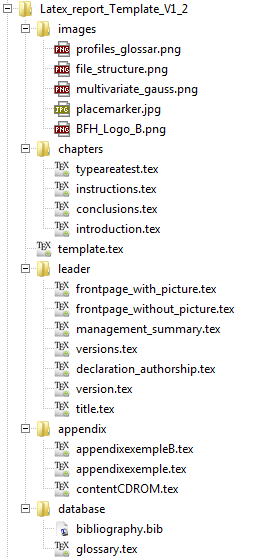
\includegraphics[scale=0.85]{images/file_structure.png}
%	\caption{File structure}
%	\label{fig:file_structure}
%\end{figure}

\section{Stainless (allgemeine Beschreibung: Struktur with pre- and postconditions, Solvers, Terminierung und mögliche Outputs)}
\label{sec:stainless}


Stainless is a framework developed by "Lab for Automated Reasoning and Analysis" (LARA) at EPFL's School of Computer and Communication Sciences. The framework is used to verify Scala programs.
It verifies statically that a program satisfies a specification given by a developer and that a program will not crash at runtime.
Stainless explores all possible input values, reports inputs for which a program fails and demonstrates counterexamples which violate a given specification.

The main functions used to write a specification are \textit{require} and \textit{ensuring}. 
A precondition should be written at the beginning of a function body with \textit{require}. Its argument is a boolean expression which corresponds to constraint for inputs of a function being verified.
A postcondition should be written after a function body with  \textit{ensuring}. It is a verification condition on an output of a function.
While compiling Stainless tries to prove that the postcondition always holds, assuming a given precondition does hold.

3 outcomes of verification with Stainless are possible: valid, unvalid and unknown. 
If the postcondition is valid, Stainless could prove that for any inputs constrained in a precondition, the postcondition always holds.
With invalid postcondition the framework could find at least one counterexample which satisfies a precondition but violates a postcondition.
Also an output unknown is possible when Stainless is unable to prove a postcondition or find a counterexample. In this case a timeout or an internal error occured.
Furthermore, it will be verified by Stainless that a precondition cannot be violated.

The following example demonstrates a simple structure of formal specification for calculating factorial.

\begin{lstlisting}[caption=Example of verifying the function calculating factorial of an integer number, captionpos=b, language=Scala]
    def factorial(n: Int): Int = {
        require(n >= 0)
        if (n == 0) {
          1
        } else {
          n * factorial(n - 1)
        }
    } ensuring(res => res >= 0)
\end{lstlisting}

The function recursively calculates factorial of an integer number. An input to the function is constrained in \textit{require} with positive value. A result of calculation should be also positive, what will be verified by Stainless.
While compiling Stainless disproves the postcondition and gives the number 17 as a counterexample. A number of type Int is a 32 bit value. That is why the function factorial of 17 causes an overflow and results to a negative value. The program would work correct by changing type of a number to BigInt.
The outcome of Stainless verification of the function factorial is shown bellow.

\begin{figure}[H]
	\centering
		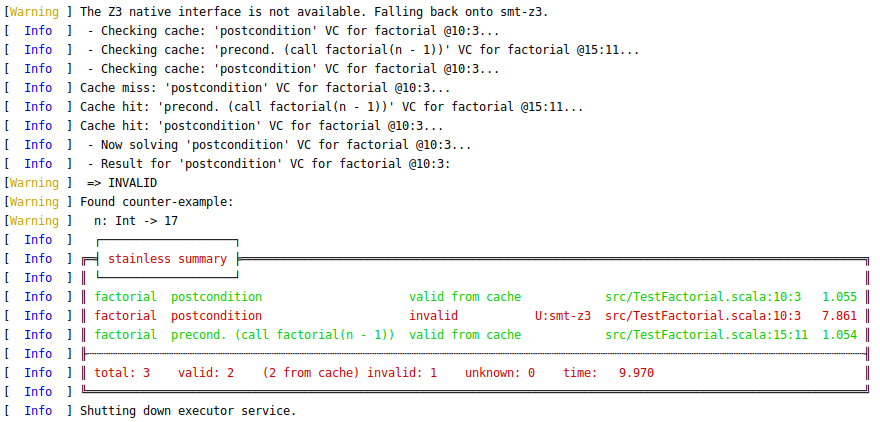
\includegraphics[scale=0.5]{images/output1.png}
	\caption{Output of Stainless verification for calculating factorial of Int number}
	\label{fig:output1}
\end{figure}


The code to be verified should be written in Pure Scala belonging to functional programming paradigm. To extend this subset of the Scala language Stainless supports also some imperative features translating them into Pure Scala concepts.
For more details about Stainless its official website can be explored. \cite{Stainless}

%\begin{table}[H]
%	\centering
%		\begin{tabular}{lll} \toprule
%			\textbf{First Name Last Name} & \textbf{E-mail} & \textbf{Function} \\ \midrule
%			Alfred Kaufmann & alfred.kaufmann@bfh.ch & Employer, Project Management, \\
%			& & Supplements, Improvements \\ \midrule
%			Fritz Dellsperger & Retired & Tips on the structure and layout \\ \midrule
%			David Burri & Contracted out & First compilation of the Template \\ \bottomrule
%		\end{tabular}
%	\caption{Contact Persons}
%	\label{tab:Contact Persons}
%\end{table}


\section{Bitcoin-S (Projekten und Packages, bitcoin-s-core, Eigenschaften zu prüfen)}
\label{sec:bitcoin_s}

%\begin{itemize}
%	\item Create a BFH Style Files
%	\item Template for the Compilation of presentations with \LaTeX{}
%\end{itemize}


